\section{WebSockets}

\subsection{Que es WebSocket y para que sirve}
\cei{WebSocket} es una tecnología que proporciona un canal de comunicación
bidireccional y full-duplex sobre un único socket TCP. Está diseñada
para ser implementada en navegadores y servidores web, pero
puede utilizarse por cualquier aplicación cliente/servidor. 

The \cei{WebSocket} specification—developed as part of the HTML5
initiative—introduced the \cei{WebSocket JavaScript interface}, which defines
a full-duplex single socket connection over which messages can be sent
between client and server. 

The WebSocket standard simplifies much of
the complexity around bi-directional web communication and connection
management.  

One of the more unique features WebSockets provide is \emph{its
ability to traverse firewalls and proxies}, a problem area for many
applications. 

Comet-style applications typically employ long-polling
as a rudimentary line of defense against firewalls and proxies.

The
technique is effective, but is not well suited for applications that
have sub-500 millisecond latency or high throughput requirements.

Plugin-based technologies such as Adobe Flash, also provide some
level of socket support, but have long been burdened with the very
proxy and firewall traversal problems that WebSockets now resolve.

A WebSocket \emph{detects the presence of a proxy server and automatically
sets up a tunnel to pass through the proxy.} 

The tunnel is established by
issuing an HTTP CONNECT statement to the proxy server, which requests
for the proxy server to open a TCP/IP connection to a specific host
and port. 

Once the tunnel is set up, communication can flow unimpeded
through the proxy. 

Since HTTP/S works in a similar fashion, secure
WebSockets over SSL can leverage the same HTTP CONNECT technique. 

Note
that WebSockets are just beginning to be supported by modern browsers
(Chrome now supports WebSockets natively). 

However, backward-compatible
implementations that enable today's browsers to take advantage of this
emerging technology are available.

En el lado del cliente, WebSocket está ya implementado en Mozilla
Firefox 8, Google Chrome 4 y Safari 5, así como la versión móvil de
Safari en el iOS 4.2.1

\subsection{Negociación del protocolo WebSocket}

Para establecer una conexión WebSocket, el cliente manda una petición de
negociación WebSocket, y el servidor manda una respuesta de negociación
WebSocket, como se puede ver en el siguiente ejemplo:

\begin{tabular}{|p{6cm}|p{6cm}|}
\begin{verbatim}
Petición del navegador al servidor:
GET /demo HTTP/1.1
Host: example.com
Connection: Upgrade
Sec-WebSocket-Key2: 12998 5 Y3 1 .P00
Sec-WebSocket-Protocol: sample
Upgrade: WebSocket
Sec-WebSocket-Key1: 4 @1 46546xW%0l 1 5
Origin: http://example.com
 
 ^n:ds[4U
\end{verbatim}
&
\begin{verbatim}
 Respuesta del servidor:
 HTTP/1.1 101 WebSocket Protocol Handshake
 Upgrade: WebSocket
 Connection: Upgrade
 Sec-WebSocket-Origin: http://example.com
 Sec-WebSocket-Location: ws://example.com/demo
 Sec-WebSocket-Protocol: sample
  
  8jKS'y:G*Co,Wxa-
\end{verbatim}
\end{tabular}

The WebSocket protocol was designed to work well with the existing
Web infrastructure. As part of this design principle, the protocol
specification defines that the WebSocket connection starts its
life as an HTTP connection, guaranteeing full backwards compatibility
with the pre-WebSocket world. 

The protocol switch from HTTP to WebSocket
is referred to as a the WebSocket handshake.

Una vez establecida, las tramas WebSocket de datos pueden empezar
a enviarse en ambos sentidos entre el cliente y el servidor en modo
full-duplex. 

Las tramas de texto pueden ser enviadas en modo full-duplex
también, en ambas direcciones al mismo tiempo. 


Tramas de datos binarios no están soportadas todavía en el API. 
  
\begin{itemize}
\item
\htmladdnormallink{About HTML5 WebSockets}{http://www.websocket.org/aboutwebsocket.html}
en 
\htmladdnormallink{http://www.websocket.org}{http://www.websocket.org}
\end{itemize}

\section{websocket/rack}

\section{Ruby y WebSockets: TCP for the Browser}

Esta sección está sacada del blog de 
\htmladdnormallink{Ilya Grigorik }{http://www.igvita.com/2009/12/22/ruby-websockets-tcp-for-the-browser/}.

WebSockets in HTML5 were designed from
the ground up to be data agnostic (binary or text) with support for
full-duplex communication. 

WebSockets are TCP for the web-browser.
They require only a single connection,
which translates into much better resource utilization for both the
server and the client. 

Likewise, WebSockets are proxy and firewall
aware, can operate over SSL and leverage the HTTP channel to
accomplish all of the above - your existing load balancers, proxies
and routers will work just fine.

\parrafo{The Server}

\begin{verbatim}
[~/sinatra/sinatra-streaming/websockets-tcp-for-the-browser(development)]$ cat server.rb
require 'em-websocket'

EventMachine::WebSocket.start(:host => "0.0.0.0", :port => 8080) do |ws|
  ws.onopen    { ws.send "Hello Client!"}
  ws.onmessage { |msg| ws.send "Pong: #{msg}" }
  ws.onclose   { puts "WebSocket closed" }
end
\end{verbatim}



\parrafo{The Client}
\begin{verbatim}
[~/sinatra/sinatra-streaming/websockets-tcp-for-the-browser(development)]$ cat index.html 
<html>
  <head>
    <script src='http://ajax.googleapis.com/ajax/libs/jquery/1.3.2/jquery.min.js'></script>
    <script>
      $(document).ready(function(){
        function debug(str){ 
          $("#debug").append("<p>"+str+"</p>"); 
        };

        ws = new WebSocket("ws://www.example.com:8080/websocket");
        ws.onmessage = function(evt) { 
          $("#msg").append("<p>"+evt.data+"</p>"); 
        };
        ws.onclose = function() { 
          debug("socket closed"); 
        };
        ws.onopen = function() {
          debug("connected...");
          ws.send("hello server");
        };
      });
    </script>
  </head>
  <body>
    <div id="debug"></div>
    <div id="msg"></div>
  </body>
</html>
\end{verbatim}
You open up a WebSocket connection simply by calling the WebSocket constructor:

\begin{verbatim}
var connection = new WebSocket('ws://html5rocks.websocket.org/echo', ['soap', 'xmpp']);
\end{verbatim}
Notice the \verb|ws:|. This is the new URL schema for WebSocket connections.
There is also \verb|wss|: for secure WebSocket connection the same way
https: is used for secure HTTP connections.

Attaching some event handlers immediately to the connection allows
you to know when the connection is opened, received incoming messages,
or there is an error.

The second argument accepts optional subprotocols. It can be a
string or an array of strings. Each string should represent a
subprotocol name and server accepts only one of passed subprotocols
in the array. Accepted subprotocol can be determined by accessing
protocol property of WebSocket object.

\begin{verbatim}
// When the connection is open, send some data to the server
connection.onopen = function () {
  connection.send('Ping'); // Send the message 'Ping' to the server
};

// Log errors
connection.onerror = function (error) {
  console.log('WebSocket Error ' + error);
};

// Log messages from the server
connection.onmessage = function (e) {
  console.log('Server: ' + e.data);
};
\end{verbatim}
As soon as we have a connection to the server (when the open event
is fired) we can start sending data to the server using the send('your
message') method on the connection object. It used to support only
strings, but in the latest spec it now can send binary messages
too. To send binary data, you can use either \verb|Blob| or \verb|ArrayBuffer|
bject.

The server might send us messages at any time. Whenever this happens
the \verb|onmessage| callback fires. The callback receives an \verb|event| object
and the actual message is accessible via the \verb|data| property.
parrafo{Ejecución}

\begin{verbatim}
[~/sinatra/sinatra-streaming/websockets-tcp-for-the-browser(development)]$ ruby server.rb
\end{verbatim}

Cuando abrimos \verb|index.html| con el navegador obtenemos una página como esta:
\begin{verbatim}
connected...

Hello Client!

Pong: hello server
\end{verbatim}

\parrafo{Véase}
\begin{enumerate}
\item 
\htmladdnormallink{Ruby and WebSockets: TCP for the Browser}{http://www.igvita.com/2009/12/22/ruby-websockets-tcp-for-the-browser/}
\item 
\htmladdnormallink{Introducing WebSockets: Bringing Sockets to the Web by Malte Ubl
and Eiji Kitamura}{http://www.html5rocks.com/en/tutorials/websockets/basics/}
2010
\item 
\htmladdnormallink{Clean, simple websockets on Sinatra example
by Austen Conrad Austen Conrad}{http://youtu.be/XVtEyilJD8M} YouTube
\end{enumerate}

\section{Una Aplicación Usando Websockets en la que Múltiples Clientes Dibujan en un Lienzo}

\parrafo{server.rb}

\begin{verbatim}
[19:36][~/srcSTW/streaming/websocketsDrawEM(master)]$ cat -n server.rb 
     1  require 'em-websocket'
     2  require 'json'
     3  require 'sinatra/base'
     4  
     5  EventMachine.run {
     6    @channel = EM::Channel.new
     7    @users = {}
     8    @messages = []
     9  
    10    EventMachine::WebSocket.start(:host => "0.0.0.0", :port => 8080) do |ws|
    11        
    12      ws.onopen {
    13        #Subscribe the new user to the channel with the callback function for the push action
    14        new_user = @channel.subscribe { |msg| ws.send msg }
    15        
    16        #Add the new user to the user list
    17        @users[ws.object_id] = new_user
    18        
    19        #Push the last messages to the user
    20        @messages.each do |message|
    21          ws.send message
    22        end
    23     }
    24  
    25      ws.onmessage { |msg|
    26        
    27        #append the message at the end of the queue
    28        @messages << msg
    29        @messages.shift if @messages.length > 10
    30  
    31        #Broadcast the message to all users connected to the channel
    32        @channel.push msg
    33      }
    34  
    35      ws.onclose { 
    36        @channel.unsubscribe(@users[ws.object_id])
    37        @users.delete(ws.object_id)
    38      }
    39    end
    40  
    41    #Run a Sinatra server for serving index.html
    42    class App < Sinatra::Base
    43      set :public_folder, settings.root
    44      
    45      get '/' do
    46        send_file 'index.html'
    47      end
    48    end
    49    App.run!
    50  } 
\end{verbatim}

\parrafo{index.html.haml}
\begin{verbatim}
!!! 5
%html
  %head
    %meta(charset="utf-8")
    %meta(content="IE=edge,chrome=1" http-equiv="X-UA-Compatible")
    %meta(name="viewport" content="width=device-width, user-scalable=0, initial-scale=1.0, maximum-scale=1.0;")  
    %link(rel="stylesheet" href="http://code.jquery.com/mobile/1.0/jquery.mobile-1.0.min.css")
    %script(type="text/javascript" src="http://code.jquery.com/jquery-1.6.4.min.js")
    %script(type="text/javascript" src="http://code.jquery.com/mobile/1.0/jquery.mobile-1.0.min.js")
    %title
      WebSockets Drawing
  %body
    :javascript
      var WebSocket = window.WebSocket || window.MozWebSocket;

      $(function() {

        var socket = new WebSocket("ws://" + location.hostname + ":8080");
       
        var currentX = 0;
        var currentY = 0;
        var lastX;
        var lastY;
        var lastReceivedX;
        var lastReceivedY;
        
        var ctx = $('#canvas')[0].getContext('2d');

        $('#canvas').bind('vmousemove',function(ev){
          ev = ev || window.event;
          currentX = ev.pageX || ev.clientX;
          currentY = ev.pageY || ev.clientY;
        });
        
        socket.onopen = function(event) {
          setInterval(function(){
            if(currentX !== lastX || currentY !== lastY){
              lastX = currentX;
              lastY = currentY;
              socket.send( JSON.stringify({x:currentX, y: currentY}) );
            }
          }, 30); // send every 300 milliseconds if position has changed
        }
        socket.onmessage = function(event) {
          var msg = $.parseJSON(event.data);
          
          ctx.beginPath();
          ctx.moveTo(lastReceivedX,lastReceivedY);
          ctx.lineTo(msg.x,msg.y);
          ctx.closePath();
          ctx.stroke();
          lastReceivedX = msg.x;
          lastReceivedY = msg.y;
        }
      });

    %div(data-role="page")
      %canvas#canvas(width='1000' height='1000')

\end{verbatim}

\parrafo{index.html}
\begin{verbatim}
<!DOCTYPE html>
<html>
  <head>
    <meta charset='utf-8' />
    <meta content='IE=edge,chrome=1' http-equiv='X-UA-Compatible' />
    <meta content='width=device-width, user-scalable=0, initial-scale=1.0, maximum-scale=1.0;' name='viewport' />
    <link href='http://code.jquery.com/mobile/1.0/jquery.mobile-1.0.min.css' rel='stylesheet' />
    <script src='http://code.jquery.com/jquery-1.6.4.min.js' type='text/javascript'></script>
    <script src='http://code.jquery.com/mobile/1.0/jquery.mobile-1.0.min.js' type='text/javascript'></script>
    <title>
      WebSockets Drawing
    </title>
  </head>
  <body>
    <script type='text/javascript'>
      //<![CDATA[
        var WebSocket = window.WebSocket || window.MozWebSocket;
        
        $(function() {
        
          var socket = new WebSocket("ws://" + location.hostname + ":8080");
         
          var currentX = 0;
          var currentY = 0;
          var lastX;
          var lastY;
          var lastReceivedX;
          var lastReceivedY;
          
          var ctx = $('#canvas')[0].getContext('2d');
        
          $('#canvas').bind('vmousemove',function(ev){
            ev = ev || window.event;
            currentX = ev.pageX || ev.clientX;
            currentY = ev.pageY || ev.clientY;
          });
          
          socket.onopen = function(event) {
            setInterval(function(){
              if(currentX !== lastX || currentY !== lastY){
                lastX = currentX;
                lastY = currentY;
                socket.send( JSON.stringify({x:currentX, y: currentY}) );
              }
            }, 30); // send every 300 milliseconds if position has changed
          }
          socket.onmessage = function(event) {
            var msg = $.parseJSON(event.data);
            
            ctx.beginPath();
            ctx.moveTo(lastReceivedX,lastReceivedY);
            ctx.lineTo(msg.x,msg.y);
            ctx.closePath();
            ctx.stroke();
            lastReceivedX = msg.x;
            lastReceivedY = msg.y;
          }
        });
      //]]>
    </script>
    <div data-role='page'>
      <canvas height='1000' id='canvas' width='1000'></canvas>
    </div>
  </body>
</html>
\end{verbatim}


\begin{figure}[htb]
\begin{center}
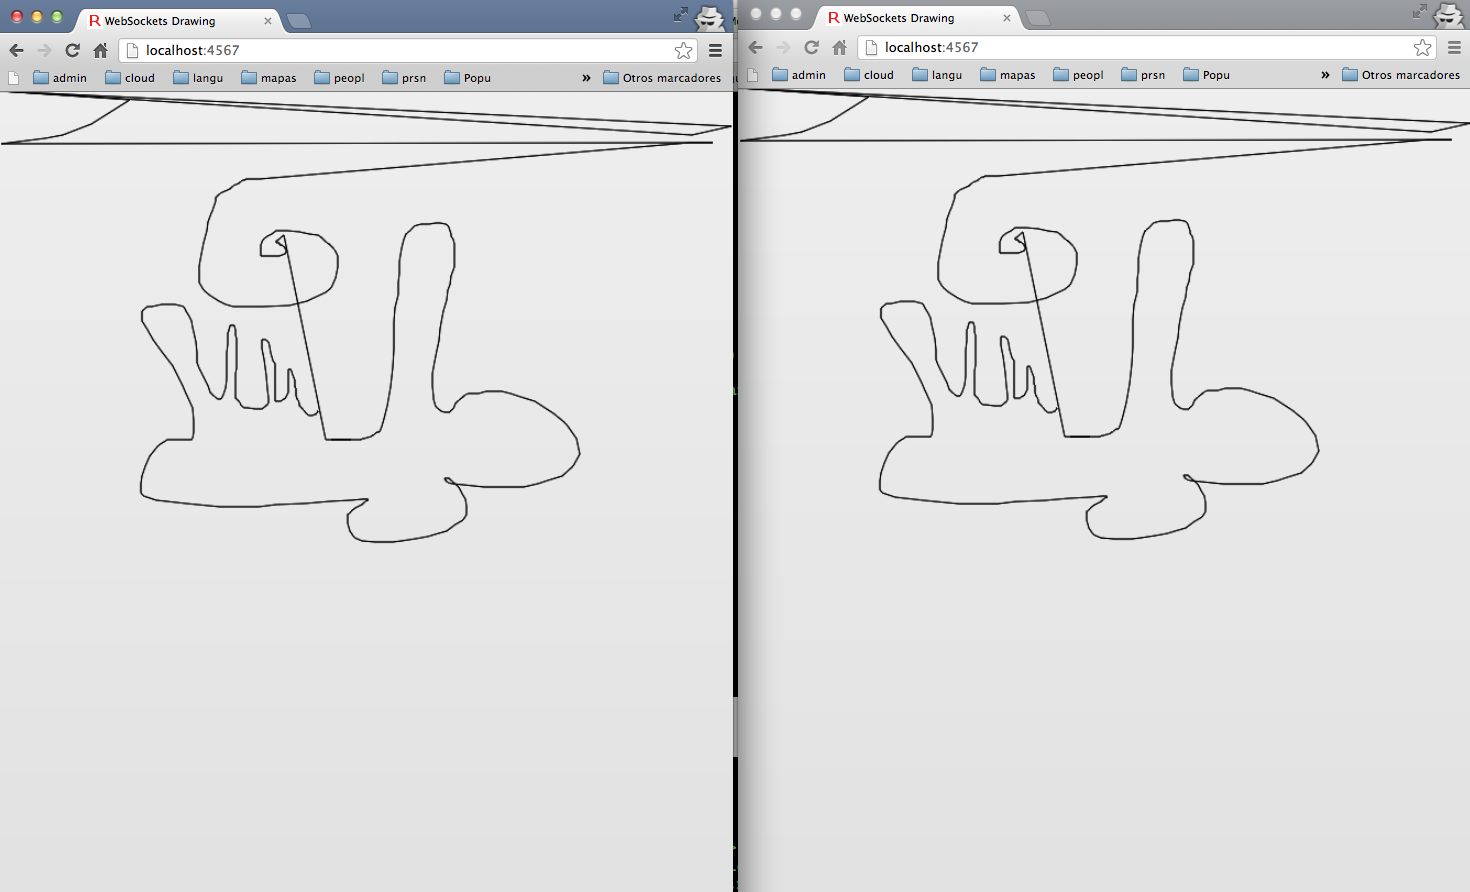
\includegraphics[scale=0.7]{sinatra/chapter2fundamentos/websockets.png}
\end{center}
\label{figure:websockets}
\caption{Múltiples clientes pueden dibujar en el lienzo}
\end{figure}

\subsection{Enlaces Relacionados}
\begin{itemize}
\item
\htmladdnormallink{A shared canvas where multiple clients can draw lines using}{http://aaltowebapps.com/websocketsDrawEM.html}
\htmladdnormallink{EM-Websocket}{https://github.com/igrigorik/em-websocket}
\item 
Este ejemplo está tomado del material del curso 
{\it Mobile Web Applications Development with HTML5}
\cite{aaltomwad}
\end{itemize}

\section{Using WebSockets on Heroku with Ruby}

\begin{enumerate}
\item 
\htmladdnormallink{Using WebSockets on Heroku with Ruby}{https://devcenter.heroku.com/articles/ruby-websockets}
\item 
\htmladdnormallink{Ruby WebSockets Chat Demo}{http://ruby-websockets-chat.herokuapp.com/}
en Heroku
\item 
\htmladdnormallink{heroku-examples / ruby-websockets-chat-demo}{https://github.com/heroku-examples/ruby-websockets-chat-demo}
en GitHub
\end{enumerate}


